\section{Comparison to Other Methods}
\subsection{Statistical Bayesian Formulation}
%%%%%%%%%%%%%%%%%%%%%%%%%%%%%%%%%%%%%%%%%%%%%%%%%%%%%%%%%%
\begin{frame}[t]

\begin{equation}\label{eq:sb_post}
    \spos\lam := \pri\lam \frac{L_\dspace (d | \lambda)}{ C },
\end{equation}
\begin{itemize}

	\item <1-> $L_\dspace$ is the likelihood function (on data)
	\item <1-> $C$ is a \emph{normalizing constant},
	\[
		C = \int_\pspace \pri\lam L_\dspace(d | \lambda) \, d\lambda.
	\]
	\item <2-> Poses a different question for which a different answer is sought:
	\item <2-> Determine a single ``true'' parameter that explains all of the observed data \cite{Smith, Concrete, Complete}
	\item <3-> We seek pull-back measure:
	\item <3-> Description of the uncertainty set that explains the variation in the observations under a given description of error
	\item <4-> It is possible to pose problems where the $\obs = L_\dspace$

\end{itemize}

\end{frame}

%%%%%%%%%%%%%%%%%%%%%%%%%%%%%%%%%%%%%%%%%%%%%%%%%%%%%%%%%%
\begin{frame}[t]
\begin{example}
Consider
\begin{equation}
u(\lambda) = \lambda^p
\end{equation}
for $p$ chosen as either 1 or 5. 

\begin{itemize}
	\item <1-> $\pri \sim U[-1,1]$. 
	\item <1-> CB: $\obs \sim \mathcal{N}(0.25,0.1^2)$
	\item <1-> SB: $d=0.25$, additive noise, $\eps \sim \mathcal{N}(0,0.1^2)$, $L_\dspace(d | \lambda) = \obs$
\end{itemize}
\end{example}
\end{frame}

%%%%%%%%%%%%%%%%%%%%%%%%%%%%%%%%%%%%%%%%%%%%%%%%%%%%%%%%%%

\begin{frame}[t]

\begin{itemize}
	\item <1,3> When $p=1$, we have $\pfpr = \frac{1}{2} = C$
	\item <1> Since $\obs\q = L_\dspace(d|\lambda)$, the posteriors agree on $\pspace$
	\item <2,3> When $p=5$, $\pfpr$ is not constant $\implies$ different posteriors
	\item <2> Push-forward of SB posterior is influenced by push-forward of prior in a manner that the CB posterior avoids
	\item <3> CB seeks to recreate the observed density
	\item <3> SB is weighted sum of likelihood and the push-forward of the prior
\end{itemize}

\begin{figure}\label{fig:comparison}
		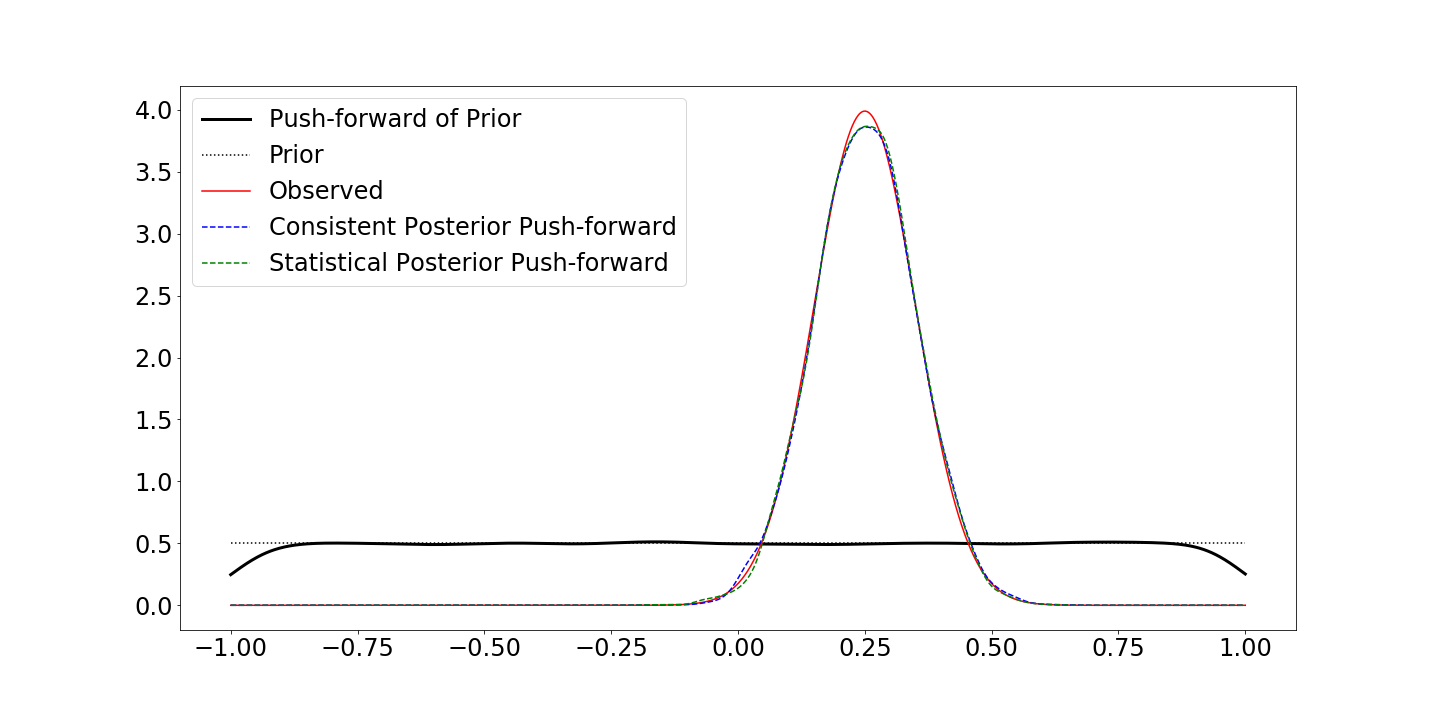
\includegraphics[width=.8\linewidth]{../images/comparison1}<1>
		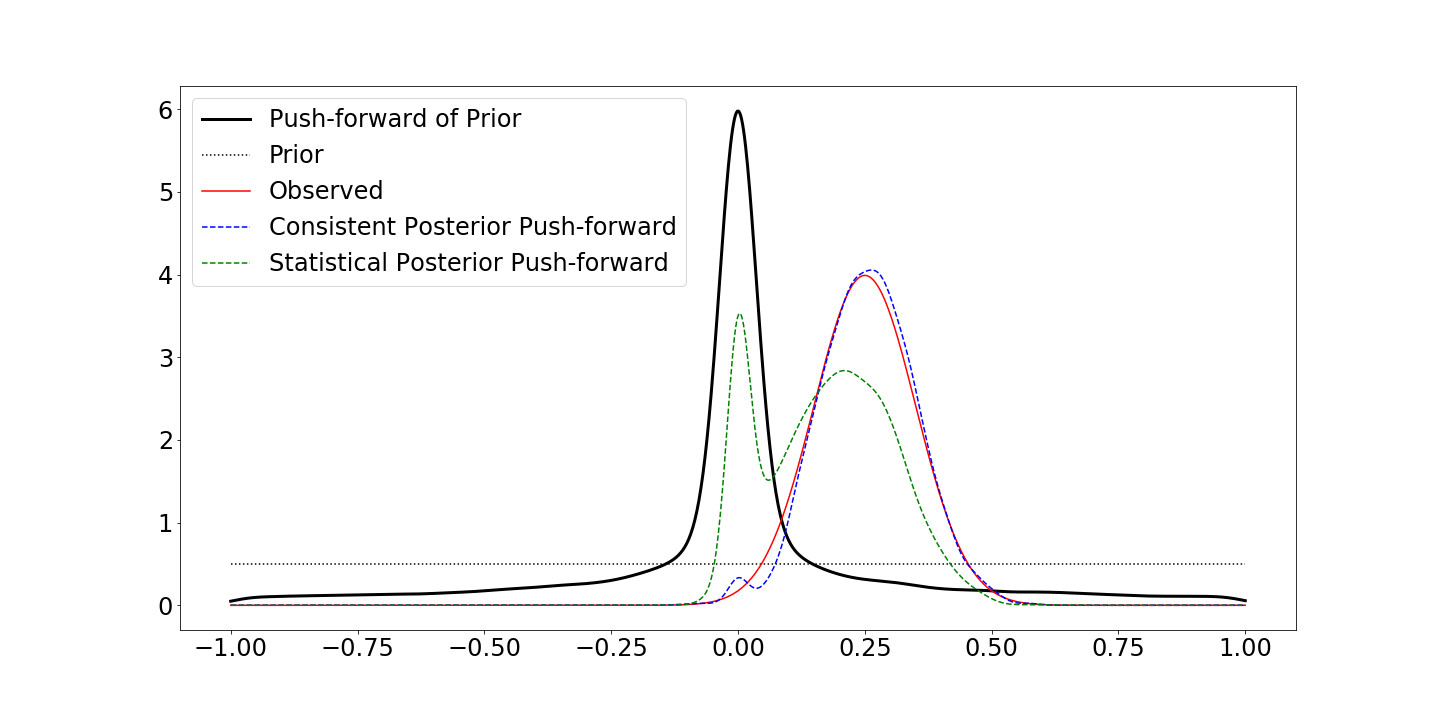
\includegraphics[width=.8\linewidth]{../images/comparison5}<2,3>
%\caption{In each plot, the black dotted line represents the prior while the solid line represents the push-forward of the prior. The push-forwards of the statistical and consistent posteriors are shown as green and blue dotted lines, respectively. The observed density/likelihood is shown as a solid red line. (Left): $p = 1$, the push-forwards of the posteriors are identical because a linear map results in a constant push-forward of a uniform prior. (Right): $p = 5$, the non-linearity of the map causes the posteriors to be different and thus the push-forwards to also be different.}
\end{figure}

\end{frame}

\subsection{Measure-Theoretic Approach: Explicit Construction}
%%%%%%%%%%%%%%%%%%%%%%%%%%%%%%%%%%%%%%%%%%%%%%%%%%%%%%%%%%
\begin{frame}[t]
\begin{itemize}[<-+->]
	\item <1-> CB framework primarily concerned with the generation of samples from a posterior
	\item <1-> In this sense, the approach is \emph{implicit} in its construction of the posterior measure
	\item <2-> Prior MT framework involved Voronoi-cell discretizations of $\pspace$
	\item <2-> Constructed set-valued approximations of the posterior measure directly
	\item <3> ``Set-based'' derivation of the posterior measure allows us to compare to approach in ~\cite{BET+14}
\end{itemize}

\end{frame}

%%%%%%%%%%%%%%%%%%%%%%%%%%%%%%%%%%%%%%%%%%%%%%%%%%%%%%%%%%
\begin{frame}[t]

\begin{figure}
\centering
	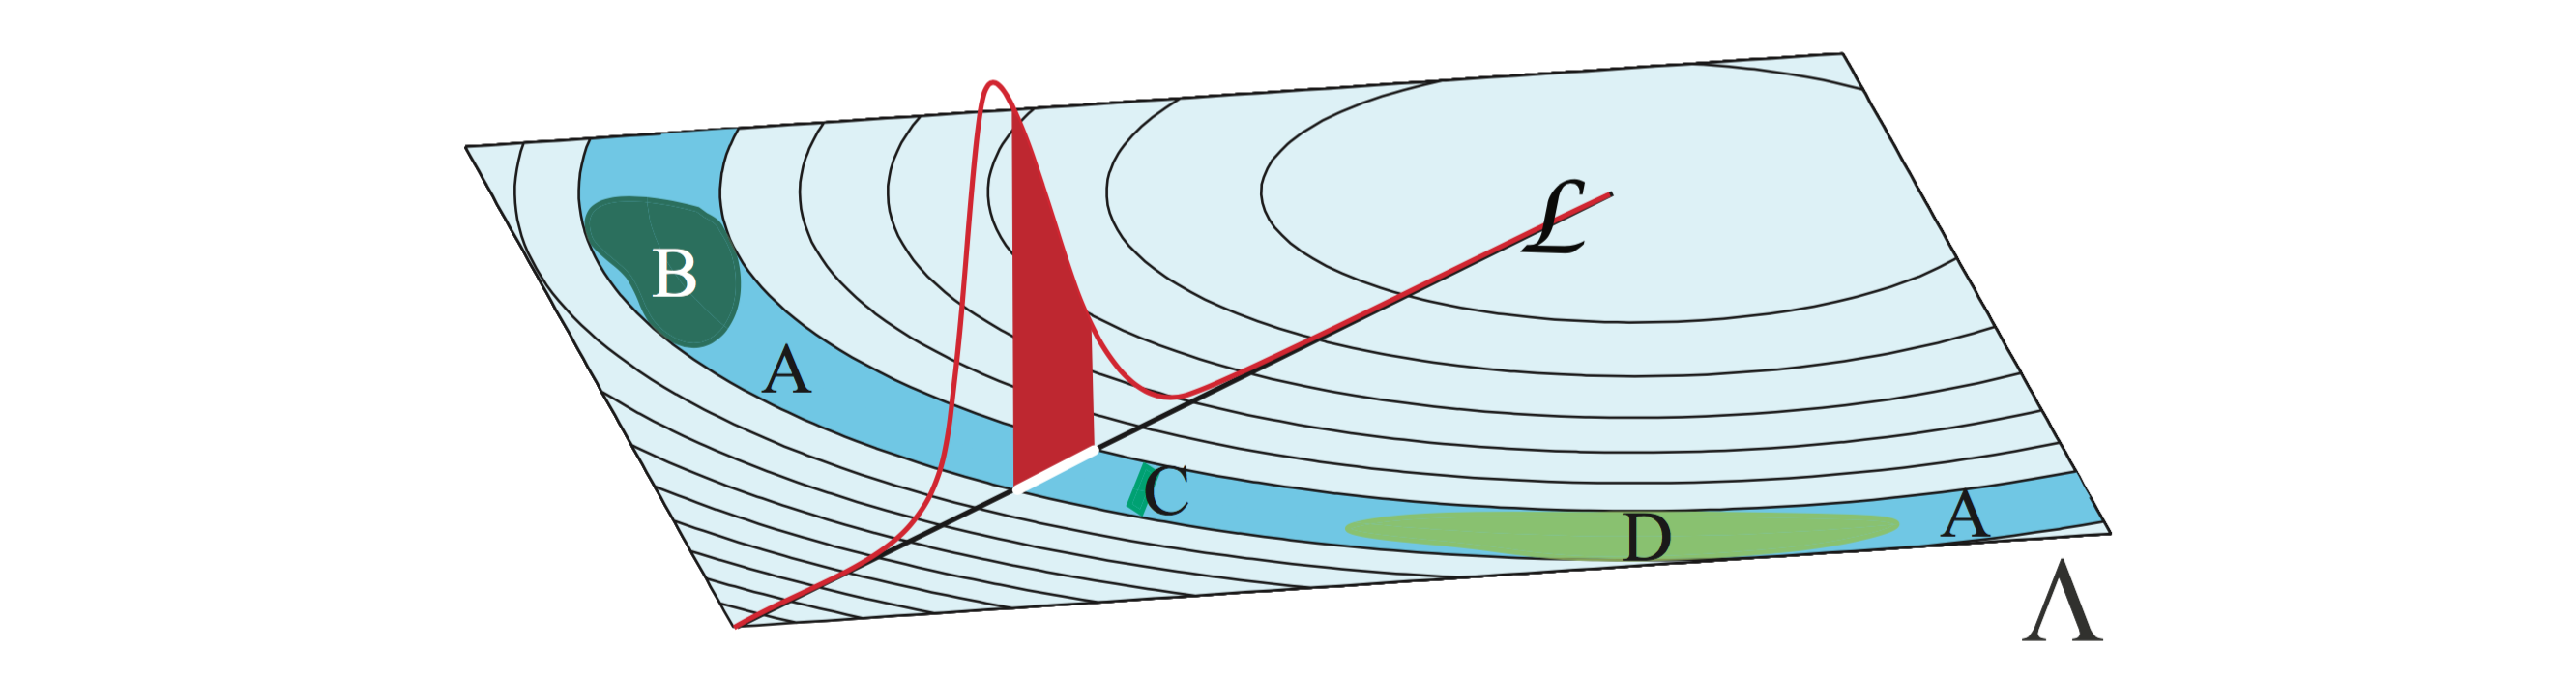
\includegraphics[width=1\textwidth]{images/troy_mt3contour}
\end{figure}
\begin{center}

{\scriptsize Figure adopted from \cite{BET+14-arxiv} and used with permission}

\tdeepred{Key Question:} Distinguish (assign probability to) events that belong to same contour. 
\end{center}
\end{frame}

%%%%%%%%%%%%%%%%%%%%%%%%%%%%%%%%%%%%%%%%%%%%%%%%%%%%%%%%%%
\begin{frame}[t]
First, we start by observing that if $A, B \subset \pspace$ such that $A = Q^{-1}(Q(B))$, then we have that $B\subset A$ (the inclusion may be proper).

Therefore, for any probability measure $P$ on $(\pspace, \pborel)$, 
\[
P(B) = P(B|A) \, P(A).
\]
If $P$ is intended to solve the inverse problem, then we are motivated to take
\[
P(A) = \Obs (Q(A)) = \Obs (B),
\]
in the above formula.
\end{frame}

%%%%%%%%%%%%%%%%%%%%%%%%%%%%%%%%%%%%%%%%%%%%%%%%%%%%%%%%%%
\begin{frame}[t]
We must now determine how to properly define $P(B|A)$. 
We leverage Bayes' Theorem~\cite{Smith} in order to utilize the prior density on contour events.

\begin{equation}\label{eq:bayes_full}
P(B|A) = \Pri(B|A) = \frac{ \Pri(A|B) \Pri(B) }{ \Pri(A) },
\end{equation}
and since $B \subset A$, $\Pri(A|B) = 1$, \eqref{eq:bayes_full} simplifies to

\begin{equation}\label{eq:bayes}
\Pri(B|A) = \frac{ \Pri(B) }{ \Pri(A) }.
\end{equation}

Since $\Pfpr$ is the push-forward of the prior, we have $\Pri(A) = \Pfpr (Q(A)) = \Pfpr \left (Q(B)\right )$, which then gives the following set-valued ``solution'' to the stochastic inverse problem:
\begin{equation}\label{eq:sip_sol_cont}
\Pos(B) := \begin{cases}
\Pri(B) \frac{ \Obs(B) }{ \Pfpr \left (Q(B)\right ) ) } & \text{ if } \Pri(B) > 0,\\
0 & \text{ otherwise}.
\end{cases}
\end{equation}

\end{frame}

%%%%%%%%%%%%%%%%%%%%%%%%%%%%%%%%%%%%%%%%%%%%%%%%%%%%%%%%%%
\begin{frame}[t]
\begin{itemize}
	\item <1-> This set-valued posterior is only a solution on certain (sub-)$\sigma$-algebras of $\pborel$, namely $\CCC_\pspace$.
	\item <1> We form explicit approximations to the posterior, e.g. as done in~\cite{BET+14, BES12, BBE11}. 
	\item <2> Ansatz is used in place of the prior:
	\item <2> It serves the same purpose to distribute probabilities in directions not informed by the QoI map.
	\item <3-> Requires an approximation of \emph{events in $\pborel$}
	\item <4-> Numerical approximation of the density $\pos$ only requires approximation of $\pfpr$
	\item <5-> Often expect the dimension of $\dspace$ to be less than the dimension of $\pspace$
	\item <5-> Possible numerical advantage for the ``implicit'' approximation given by the posterior probability density function
\end{itemize}
\end{frame}

